\chapter{Wstęp}
\label{chap:wstep}

Automatyczna Transkrypcja Muzyczna (ATM) (\english{Automatic Music Transcription}) stanowi jedno z kluczowych i jednocześnie najbardziej złożonych zadań w dziedzinie komputerowej analizy muzyki.
W swej istocie, ATM jest procesem konwersji sygnału akustycznego, będącego fizyczną manifestacją muzyki, na jego symboliczną, strukturalną reprezentację \autocite{KlapuriDavy2006SignalProcessing,Benetos2019AutomaticMusicTranscription}.
Celem tego procesu jest przekształcenie ciągłego sygnału audio w dyskretny zestaw symboli muzycznych, takich jak tradycyjne nuty określające wysokość i czas trwania dźwięku, lub – co jest przedmiotem szczególnego zainteresowania w niniejszej pracy – w zapis tabulaturowy.
Interdyscyplinarny charakter Automatycznej Transkrypcji Muzycznej jest niezaprzeczalny, gdyż skuteczna realizacja jej zadań wymaga integracji wiedzy i metodologii pochodzących z wielu, pozornie odległych, dziedzin nauki i techniki.
Do najważniejszych z nich należą:
\begin{itemize}
\item \textbf{Cyfrowe Przetwarzanie Sygnałów (CPS)} (\english{Digital Signal Processing – DSP}): Dostarcza ono fundamentalnych narzędzi do analizy, transformacji i manipulacji sygnałem audio w dziedzinie czasu i częstotliwości.
Techniki takie jak filtracja, analiza spektralna czy transformacje czasowo-częstotliwościowe są nieodzowne w procesie ekstrakcji informacji z surowego sygnału dźwiękowego \autocite{KlapuriDavy2006SignalProcessing}.
Zaawansowane metody CPS pozwalają na wstępne przygotowanie sygnału, redukcję szumów oraz identyfikację podstawowych cech akustycznych, które następnie mogą być interpretowane w kontekście muzycznym.
Przykładem fundamentalnego narzędzia CPS, ilustrującego przejście z dziedziny czasu do dziedziny częstotliwości, jest dyskretna transformata Fouriera (DFT) (\english{Discrete Fourier Transform}).
Dla skończonego ciągu próbek sygnału $x_n$ o długości N, jej k-ty współczynnik $X_k$ jest zdefiniowany jako:
\begin{equation}
X_k = \sum_{n=0}^{N-1} x_n \cdot e^{-i\frac{2\pi}{N}kn}
\label{eq:dft}
\end{equation}
gdzie $n$ jest indeksem próbki w dziedzinie czasu, $k$ jest indeksem częstotliwości, a $i$ jest jednostką urojoną.
Wzór ten jest podstawą wielu algorytmów analizy częstotliwościowej stosowanych w ATM.
\item \textbf{Rozpoznawanie Wzorców} (\english{Pattern Recognition}) oraz \textbf{Uczenie Maszynowe (UM)} (\english{Machine Learning – ML}): Te dziedziny odgrywają kluczową rolę w identyfikacji złożonych struktur muzycznych, takich jak pojedyncze nuty, akordy, rytmy czy motywy melodyczne, w często zaszumionym i polifonicznym sygnale audio \autocite{Benetos2019AutomaticMusicTranscription}.
Współczesne systemy ATM w coraz większym stopniu opierają się na zaawansowanych modelach uczenia maszynowego, w szczególności na sieciach neuronowych i głębokim uczeniu (\english{Deep Learning}), które potrafią automatycznie uczyć się hierarchicznych reprezentacji cech muzycznych bezpośrednio z danych \autocite{BurletHindle2017IsolatedGuitarTranscription}.
Dynamiczny rozwój w obszarze głębokiego uczenia bezpośrednio przekłada się na postępy w ATM, umożliwiając tworzenie modeli zdolnych do przetwarzania coraz bardziej skomplikowanych sygnałów muzycznych z niespotykaną dotąd dokładnością.
\item \textbf{Sztuczna Inteligencja (SI)} (\english{Artificial Intelligence – AI}): Jako szersza dziedzina, obejmuje ona uczenie maszynowe, ale także inne aspekty, takie jak reprezentacja wiedzy muzycznej oraz procesy poznawcze związane z percepcją i wnioskowaniem w kontekście muzycznym \autocite{Benetos2019AutomaticMusicTranscription}.
Rozwój SI dostarcza ram koncepcyjnych i narzędziowych dla budowy inteligentnych systemów transkrypcji.
\item \textbf{Muzykologia}: Dostarcza niezbędnej wiedzy teoretycznej o strukturze muzyki, notacji, harmonii, rytmie oraz praktykach wykonawczych \autocite{Holzapfel2019Ethnomusicology}.
Zrozumienie zasad muzycznych jest kluczowe nie tylko dla interpretacji wyników generowanych przez systemy ATM, ale również dla projektowania algorytmów, które uwzględniają kontekst muzyczny i dążą do tworzenia transkrypcji użytecznych z perspektywy muzykologicznej i wykonawczej.
\end{itemize}

Potencjalne obszary zastosowań systemów ATM są szerokie i różnorodne, co podkreśla ich rosnące znaczenie zarówno w badaniach naukowych, jak i w praktyce muzycznej.
Do najważniejszych aplikacji należą: wsparcie w edukacji muzycznej, na przykład poprzez tworzenie systemów do automatyzacji ćwiczeń gry na instrumencie, analizę postępów ucznia czy generowanie spersonalizowanych materiałów dydaktycznych \autocite{Benetos2019AutomaticMusicTranscription}.
Systemy ATM mogą również znacząco ułatwić proces tworzenia i aranżacji muzyki, na przykład poprzez wspieranie modyfikacji i rearanżacji istniejących utworów \autocite{ArndtLi2012AutomatedTranscription}.
Dla producentów muzycznych, ATM oferuje narzędzia do wizualizacji treści muzycznej i inteligentnej edycji nagrań \autocite{Benetos2019AutomaticMusicTranscription}.
Ponadto, technologie te są wykorzystywane w systemach wyszukiwania i kategoryzacji muzyki w dużych zbiorach danych, na przykład poprzez umożliwienie wyszukiwania utworów na podstawie ich melodii, harmonii czy rytmu \autocite{Benetos2019AutomaticMusicTranscription}.
Tytuł niniejszej pracy, ,,Przekształcanie nagrań dźwiękowych na zapis nutowy'', odnosi się do centralnego problemu ATM.
Należy jednak podkreślić, że termin ,,zapis nutowy'' jest pojęciem szerokim, obejmującym różnorodne systemy notacji muzycznej.
W kontekście niniejszego opracowania, szczególna uwaga zostanie poświęcona specyficznej formie zapisu, jaką jest tabulatura gitarowa.
Tabulatura, w odróżnieniu od tradycyjnej notacji nutowej skupiającej się \english{primarnie} na wysokości i czasie trwania dźwięku, jest graficzną reprezentacją wskazującą bezpośrednio pozycje palców na gryfie instrumentu – konkretne struny i progi, które należy nacisnąć, aby uzyskać pożądany dźwięk \autocite{Wiggins2019TabCNN}.
\begin{figure}[htbp]
\centering
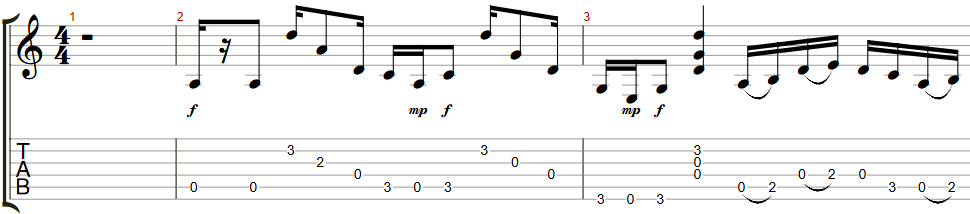
\includegraphics[width=0.9\textwidth]{fig/fig_1_1.png}
\caption{Porównanie fragmentu zapisu nutowego i odpowiadającej mu tabulatury gitarowej dla motywu muzycznego.}
\label{fig:porownanie_nuty_tabulatura}
\end{figure}

Wybór tabulatury jako docelowej formy zapisu w tej pracy nie jest przypadkowy.
Wynika on ze specyfiki gitary jako instrumentu oraz z ogromnej popularności tej formy notacji wśród gitarzystów \autocite{Wiggins2019TabCNN}.
Rosnąca popularność tabulatur, często udostępnianych online, stwarza specyficzne zapotrzebowanie na systemy ATM zdolne do generowania tego właśnie formatu.
Nie jest to jedynie kwestia preferencji użytkowników; tabulatura często zawiera informacje o charakterze performatywnym, takie jak konkretne opalcowanie czy użycie technik gitarowych, których brakuje w standardowej notacji nutowej.
Skuteczne systemy ATM generujące tabulatury mogą zatem zdemokratyzować proces nauki gry na gitarze oraz tworzenia muzyki, obniżając barierę wejścia dla osób, które nie posługują się biegle tradycyjnym zapisem nutowym, ale rozumieją intuicyjny charakter tabulatury.
Ten wybór stanowi naturalne przejście do dalszych, bardziej szczegółowych rozważań przedstawionych w kolejnych rozdziałach pracy.

\section{Osadzenie problemu w dziedzinie naukowej}
\label{sec:osadzenie_problemu}

Przedmiotem niniejszej pracy jest zagadnienie automatycznej transkrypcji muzyki gitarowej do postaci tabulatury, co sytuuje ją w szerokim kontekście badań prowadzonych w ramach dziedziny naukowej znanej jako \english{Music Information Retrieval (MIR)}.
MIR, czyli komputerowe pozyskiwanie informacji muzycznej, jest interdyscyplinarnym polem badawczym zajmującym się analizą, przetwarzaniem, wyszukiwaniem, organizacją i dostępem do informacji zawartej w muzyce, zarówno w jej formie akustycznej, jak i symbolicznej.
Obserwowany w ostatnich dekadach gwałtowny wzrost ilości dostępnych cyfrowych treści muzycznych, na przykład w ramach cyfrowych bibliotek muzycznych i serwisów streamingowych \autocite{Benetos2019AutomaticMusicTranscription}, generuje rosnące zapotrzebowanie na zautomatyzowane narzędzia do ich analizy.
Narzędzia te są niezbędne do efektywnego zarządzania ogromnymi repozytoriami muzyki, ich przeszukiwania, kategoryzacji oraz personalizacji dostępu dla użytkowników.
ATM jest jednym z kluczowych zadań w ramach MIR, umożliwiającym transformację sygnału audio na bogatszą, symboliczną reprezentację, która może być dalej przetwarzana i analizowana.
Szczególną uwagę w kontekście niniejszej pracy należy poświęcić wyzwaniom związanym z transkrypcją muzyki gitarowej.
Gitara, będąca instrumentem niezwykle popularnym i wszechstronnym, wykorzystywanym w niemal każdym gatunku muzycznym, stawia przed systemami ATM szereg specyficznych trudności:
\begin{itemize}
\item \textbf{Polifoniczność}: Gitara jest instrumentem polifonicznym, co oznacza zdolność do jednoczesnego wydawania wielu dźwięków (standardowo do sześciu, po jednym na każdej strunie) \autocite{BurletHindle2017IsolatedGuitarTranscription}.
Nakładanie się składowych harmonicznych wielu jednocześnie brzmiących dźwięków w sygnale audio znacząco komplikuje proces ich separacji i identyfikacji.
\begin{figure}[htbp]
\centering
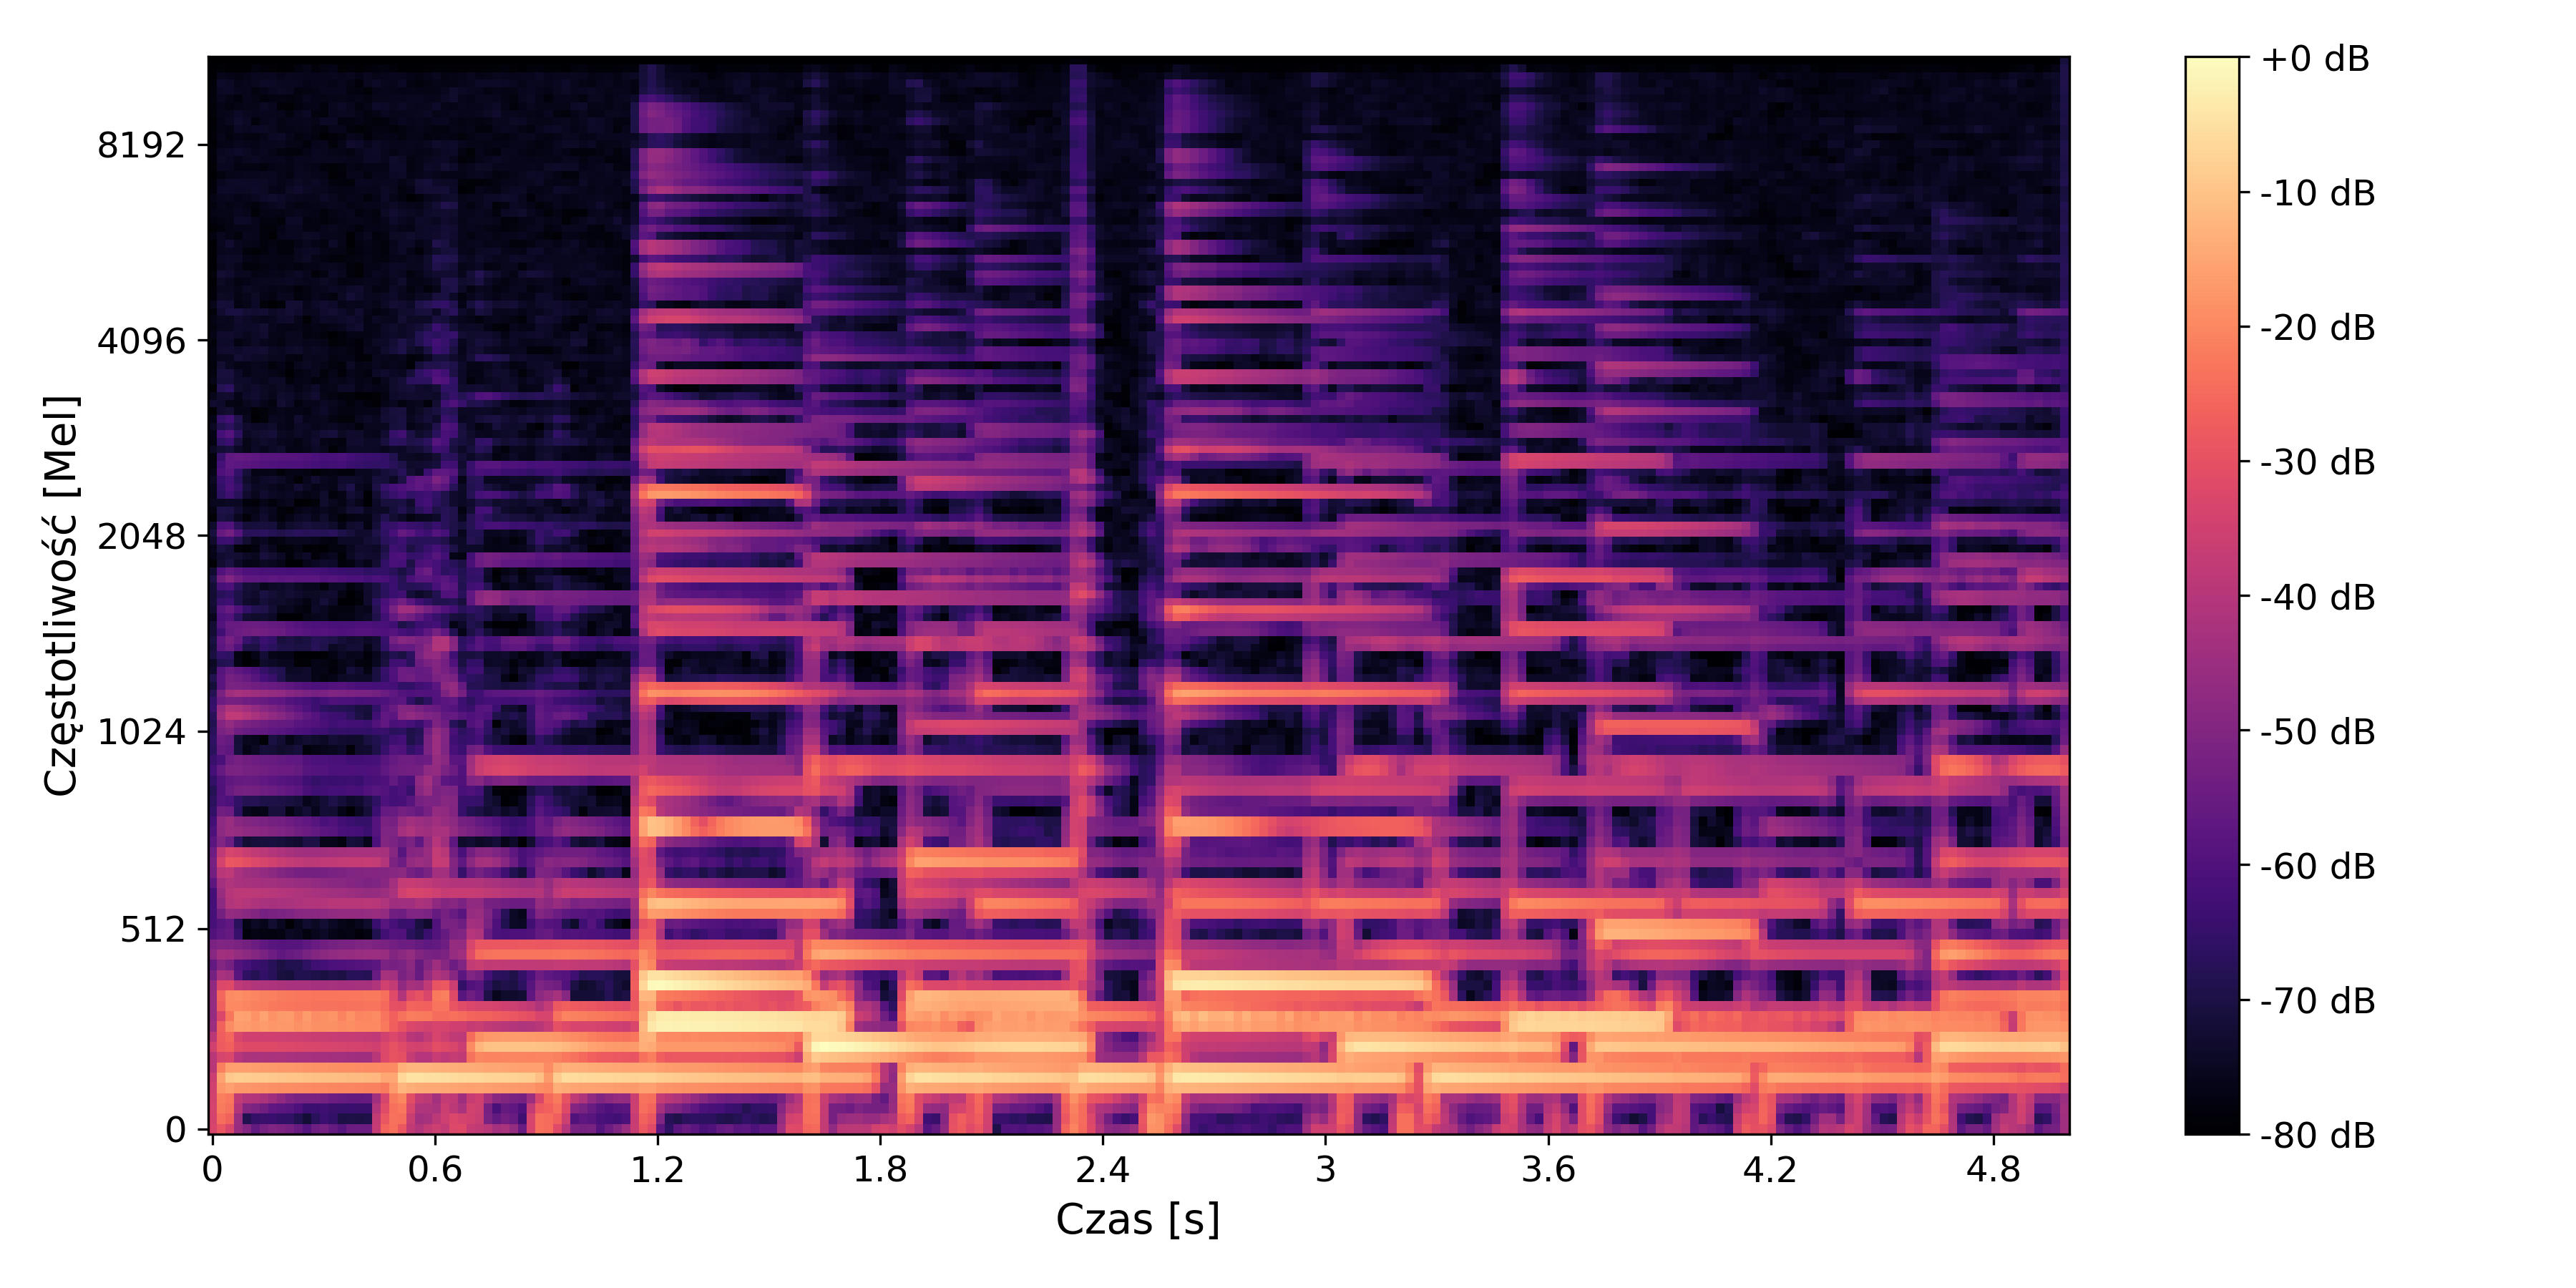
\includegraphics[width=\textwidth]{fig/fig_1_2.png}
\caption{Schematyczny przykład spektrogramu polifonicznego sygnału gitarowego, ukazujący nakładające się struktury harmoniczne (prążki reprezentujące częstotliwość podstawową i jej alikwoty) dla kilku jednocześnie brzmiących nut.}
\label{fig:spektrogram_polifoniczny}
\end{figure}
\item \textbf{Bogactwo technik artykulacyjnych}: Gitarzyści wykorzystują szeroki wachlarz technik artykulacyjnych, takich jak podciąganie strun (\english{bending}), ślizgi (\english{sliding}), młoteczkowanie (\english{hammer-on}), odrywanie (\english{pull-off}), wibrato (\english{vibrato}) czy tłumienie strun dłonią (\english{palm-muting}).
Każda z tych technik w unikalny sposób modyfikuje charakterystykę sygnału akustycznego (np. jego wysokość, amplitudę, barwę w czasie) i jest kluczowa dla wiernej transkrypcji, zwłaszcza do formatu tabulatury, który często zawiera symbole oznaczające te techniki.
\item \textbf{Duża zmienność barwy dźwięku (\english{timbre})}: Barwa dźwięku gitary jest niezwykle zróżnicowana i zależy od wielu czynników, takich jak typ instrumentu (np. gitara akustyczna, klasyczna, elektryczna), rodzaj użytych strun, sposób ich pobudzenia (kostką, palcami), a w przypadku gitar elektrycznych – od ustawień wzmacniacza i zastosowanych efektów gitarowych \autocite{Wiggins2019TabCNN}.
Ta duża wariabilność barwy stanowi poważne wyzwanie dla modeli uczenia maszynowego, które muszą generalizować swoją wiedzę na różne instancje dźwięków gitarowych.
\item \textbf{Identyczność wysokości dźwięku na różnych strunach i progach}: Jedną z charakterystycznych cech gitary jest możliwość zagrania dźwięku o tej samej wysokości w wielu różnych pozycjach na gryfie (tj. na różnych kombinacjach struny i progu) \autocite{Wiggins2019TabCNN}.
O ile dla tradycyjnej notacji nutowej ta wieloznaczność nie jest problemem, o tyle dla generowania tabulatury, która musi precyzyjnie wskazać miejsce zagrania dźwięku, jest to fundamentalne wyzwanie.
Wybór odpowiedniej pozycji często zależy od kontekstu muzycznego, grywalności (łatwości wykonania) i preferencji wykonawcy.
\end{itemize}

Pomimo znaczących postępów, jakie dokonały się w dziedzinie ATM w ostatnich latach, zwłaszcza dzięki zastosowaniu zaawansowanych technik uczenia maszynowego, istniejące systemy wciąż borykają się z ograniczeniami, prowadzącymi do typowych błędów, takich jak pomyłki oktawowe, niepoprawne detekcje nut czy niedokładności czasowe \autocite{Benetos2019AutomaticMusicTranscription}.
Człowiek, dokonując transkrypcji, opiera się nie tylko na percepcji sygnału akustycznego, ale również na swojej rozległej wiedzy muzycznej, znajomości teorii muzyki, konwencji stylistycznych oraz kontekstu kulturowego.
Maszyny, mimo coraz doskonalszych algorytmów, wciąż mają trudności z pełnym uwzględnieniem tych aspektów \autocite{Holzapfel2019Ethnomusicology}.
Ograniczenia te są szczególnie widoczne w przypadku transkrypcji muzyki polifonicznej, wykonywanej na instrumentach o złożonej charakterystyce akustycznej, takich jak gitara \autocite{BurletHindle2017IsolatedGuitarTranscription}.
Niedoskonałość obecnych systemów, zwłaszcza w kontekście precyzyjnego odwzorowania niuansów wykonawczych gitary i generowania użytecznych, grywalnych tabulatur, stanowi silny impuls do poszukiwania nowych, bardziej efektywnych rozwiązań.
Ta luka badawcza jest główną motywacją do podjęcia tematu niniejszej pracy.
Popularność gitary oraz ogromna ilość dostępnych nagrań gitarowych, często pozbawionych wiarygodnych transkrypcji, tworzą naturalne zapotrzebowanie na narzędzia MIR, w tym ATM.
Postępy w tej dziedzinie mogą z kolei stymulować dalsze tworzenie i udostępnianie muzyki, tworząc pozytywną pętlę sprzężenia zwrotnego.
Co więcej, rozwój precyzyjnych systemów ATM dla gitary może odegrać istotną rolę w dokumentacji i archiwizacji unikalnych stylów gitarowych oraz technik wykonawczych, stanowiących ważne elementy dziedzictwa kulturowego.
Otwartym problemem pozostaje również ocena jakości transkrypcji, zwłaszcza w kontekście tabulatur, co zostało zasygnalizowane w literaturze \autocite{Zang2023SynthTab}.

\section{Cel pracy}
\label{sec:cel_pracy}

Głównym celem niniejszej pracy magisterskiej jest zaprojektowanie, implementacja oraz weryfikacja eksperymentalna systemu służącego do automatycznej transkrypcji polifonicznych nagrań audio gitary na zapis tabulaturowy.
Kluczowym elementem realizacji tego celu jest wykorzystanie publicznie dostępnego zbioru danych Guitarset.
Zbiór ten, opisany i wykorzystany w badaniach nad transkrypcją gitarową (np. \autocite{Wiggins2019TabCNN}), został specjalnie przygotowany do tego celu i charakteryzuje się unikalnymi cechami, takimi jak dostarczanie nagrań heksafonicznych (sygnału z każdej struny osobno) wraz z precyzyjnymi adnotacjami dotyczącymi wysokości dźwięku, czasu jego trwania oraz, co szczególnie istotne, informacji o strunie i progu, na którym dany dźwięk został zagrany \autocite{Wiggins2019TabCNN}.
Wybór zbioru Guitarset jest zatem nieprzypadkowy; jego struktura bezpośrednio adresuje problem niejednoznaczności przypisania dźwięku do konkretnej pozycji na gryfie, co jest fundamentalne przy tworzeniu wiarygodnych danych uczących i testowych dla zadania generowania tabulatury.
System opracowany w ramach tej pracy ma dążyć do precyzyjnego odwzorowania partii gitarowych w formie tabulatury.
Oznacza to nie tylko poprawną identyfikację atrybutów muzycznych takich jak wysokość i czas trwania dźwięków, ale przede wszystkim ich prawidłowe przypisanie do odpowiednich strun i progów na gryfie gitary.
Dążenie do precyzji obejmuje również próbę radzenia sobie z wyzwaniami specyficznymi dla transkrypcji gitary, które zostały omówione w poprzednim podrozdziale, takimi jak wysoki stopień polifonii, zróżnicowane techniki artykulacyjne oraz konieczność generowania tabulatury uwzględniającej aspekty grywalności.
Realizacja tak zdefiniowanego celu pracy, czyli stworzenie efektywnego systemu transkrypcji nagrań gitarowych do postaci tabulatury, może przyczynić się do powstania nowych narzędzi wspierających kreatywność i edukację gitarzystów.
Przykładowo, taki system mógłby służyć do automatycznego generowania tabulatur z improwizowanych fragmentów muzycznych, ułatwiać analizę złożonych partii gitarowych znanych wykonawców, czy też stanowić cenne wsparcie w procesie nauki gry na instrumencie.

\section{Zakres pracy}
\label{sec:zakres_pracy}

Realizacja postawionego celu badawczego obejmuje następujące, kluczowe etapy:
\begin{itemize}
\item Przeprowadzenie szczegółowej analizy literatury naukowej dotyczącej automatycznej transkrypcji muzycznej, ze szczególnym naciskiem na metody stosowane w transkrypcji muzyki gitarowej, specyfikę sygnału generowanego przez ten instrument oraz różne aspekty notacji tabulaturowej, w tym jej strukturę i konwencje zapisu.
\item Zaprojektowanie architektury systemu do automatycznej transkrypcji, która będzie uwzględniać specyfikę zadania, charakterystykę danych wejściowych (polifoniczne nagrania gitary akustycznej) i wyjściowych (zapis tabulaturowy) oraz dostępne narzędzia i technologie, w tym potencjalne wykorzystanie modeli głębokiego uczenia.
\item Implementacja kluczowych modułów składowych systemu, obejmujących co najmniej:
\begin{itemize}
\item Moduł przetwarzania wstępnego sygnału audio (\english{audio preprocessing}), mający na celu przygotowanie sygnału do dalszej analizy, np. poprzez normalizację, segmentację czy redukcję szumów.
\item Moduł ekstrakcji cech akustycznych (\english{acoustic feature extraction}), odpowiedzialny za przekształcenie przetworzonego sygnału audio w reprezentację numeryczną, która efektywnie koduje informacje istotne dla rozpoznawania dźwięków gitarowych i ich atrybutów.
Rozważone zostaną zarówno klasyczne cechy akustyczne \autocite{KlapuriDavy2006SignalProcessing}, jak i cechy uzyskiwane automatycznie z wykorzystaniem metod głębokiego uczenia \autocite{BurletHindle2017IsolatedGuitarTranscription}.
\item Moduł predykcyjny, oparty na wybranych technikach uczenia maszynowego, którego zadaniem będzie generowanie sekwencji zdarzeń tabulatu\-rowych (struna, próg, czas rozpoczęcia, czas trwania) na podstawie wyekstra\-howanych cech akustycznych.
\end{itemize}
\item Adaptacja i wykorzystanie publicznie dostępnego zbioru danych Guitarset, opisanego m.in. w \autocite{Wiggins2019TabCNN}, do procesu trenowania, walidacji oraz testowania opracowanego systemu.
Etap ten będzie obejmował przygotowanie danych do formatu wymaganego przez zaimplementowany model, w tym potencjalne techniki augmentacji danych w celu zwiększenia robustości modelu.
\item Zdefiniowanie i dobór odpowiednich metryk oceny jakości transkrypcji tabulaturowej.
Metryki te muszą uwzględniać nie tylko poprawność wykrytych nut pod względem ich wysokości, czasu rozpoczęcia i czasu trwania, ale także, co kluczowe dla tego zadania, poprawność przypisania poszczególnych dźwięków do konkretnych strun i progów gitary.
\item Przeprowadzenie kompleksowych badań eksperymentalnych mających na celu weryfikację skuteczności i wydajności zaproponowanego rozwiązania.
Wyniki uzyskane przez system będą porównywane z adnotacjami referencyjnymi ze zbioru Guitarset oraz, w miarę możliwości, z wynikami innych istniejących metod lub systemów transkrypcji gitarowej, aby ocenić postęp względem aktualnego stanu wiedzy (\english{state-of-the-art}) \autocite{Benetos2019AutomaticMusicTranscription}.
\item Dokładna analiza uzyskanych wyników eksperymentalnych, obejmująca zarówno ocenę ilościową (na podstawie zdefiniowanych metryk), jak i jakościową (np. poprzez analizę typowych błędów popełnianych przez system).
Na tej podstawie zostaną zidentyfikowane mocne i słabe strony opracowanego systemu oraz sformułowane wnioski końcowe i rekomendacje dotyczące potencjalnych ulepszeń oraz dalszych kierunków badań w tej dziedzinie.
\end{itemize}
Niniejsza praca będzie koncentrować się na rozwiązaniu konkretnego problemu o charakterze naukowo-badawczym.
Osiągnięcie tego celu nastąpi poprzez opracowanie innowacyjnego rozwiązania technicznego, jakim jest system do automatycznej transkrypcji gitarowej na tabulaturę, oraz udokumentowanie kompetencji inżynierskich autora w zakresie projektowania, implementacji i weryfikacji systemów opartych na przetwarzaniu sygnałów i uczeniu maszynowym.
Przedstawiony zakres pracy odzwierciedla standardowy cykl życia projektu badawczo-rozwojowego w dziedzinie uczenia maszynowego, co zapewnia metodyczne i kompleksowe podejście do postawionego problemu.
Szczególny nacisk położony na adaptację zbioru Guitarset oraz zdefiniowanie specyficznych metryk oceny jakości transkrypcji tabulaturowej wskazuje na potencjalny wkład pracy nie tylko w sam system, ale również w metodykę badań nad transkrypcją gitarową.

\section{Zwięzła charakterystyka rozdziałów}
\label{sec:charakterystyka_rozdzialow}

Struktura niniejszej pracy magisterskiej została zaprojektowana w sposób umożliwiający logiczne i spójne przedstawienie podjętej problematyki, przeprowadzonych badań oraz uzyskanych wyników.
Poniżej przedstawiono zwięzłą charakterystykę poszczególnych rozdziałów:
\begin{description}
\item[Rozdział 1 (Wstęp)] Prezentowany rozdział. Wprowadza on w problematykę pracy, definiuje automatyczną transkrypcję muzyczną (ATM) i jej specyfikę w kontekście gitary i tabulatury.
Osadza problem w dziedzinie naukowej \english{Music Information Retrieval (MIR)}, omawia wyzwania związane z transkrypcją gitarową.
Formułuje cel i zakres pracy, przedstawia strukturę kolejnych rozdziałów oraz jednoznacznie określa wkład autora.
\item[Rozdział 2 (Analiza Tematu)] Rozdział ten poświęcony będzie dogłębnemu przedstawieniu podstaw teoretycznych niezbędnych do zrozumienia problematyki pracy.
Omówione zostaną fundamentalne pojęcia dotyczące dźwięku muzycznego, jego cyfrowej reprezentacji \autocite{KlapuriDavy2006SignalProcessing} oraz podstawowych metod jego analizy.
Następnie, zaprezentowane zostaną ogólne zagadnienia związane z automatyczną transkrypcją muzyczną, po czym szczegółowa uwaga zostanie skupiona na specyfice transkrypcji gitarowej.
Dokładnie scharakteryzowany zostanie sygnał gitary, jego cechy akustyczne oraz notacja tabulaturowa.
Rozdział ten płynnie przejdzie do sprecyzowania problematyki badawczej podejmowanej w niniejszej pracy.
\item[Rozdział 3 (Przedmiot Pracy)] W tym rozdziale opisane zostanie autorskie rozwiązanie problemu automatycznej transkrypcji polifonicznych nagrań gitarowych na zapis tabulaturowy.
Zaprezentowana zostanie szczegółowa architektura zaimplementowanego systemu, wraz z opisem poszczególnych jego modułów.
Dokładnie scharakteryzowany zostanie wykorzystany zbiór danych Guitarset, którego cechy i zastosowanie w badaniach opisano m.in. w \autocite{Wiggins2019TabCNN}, oraz proces jego adaptacji na potrzeby systemu. Uzasadniony zostanie również wybór zastosowanych metod przetwarzania sygnału, ekstrakcji cech, algorytmów uczenia maszynowego oraz wykorzystanych narzędzi programistycznych.
\item[Rozdział 4 (Badania)] Ten rozdział będzie poświęcony prezentacji metodyki oraz wyników przeprowadzonych badań eksperymentalnych.
Opisane zostanie środowisko badawcze, sposób przygotowania danych testowych oraz zdefiniowane metryki oceny jakości transkrypcji.
Uzyskane wyniki zostaną zaprezentowane w sposób ilościowy (np. w postaci tabel i wykresów) oraz jakościowy.
Następnie wyniki te zostaną poddane szczegółowej analizie i dyskusji, w tym identyfikacji typowych błędów popełnianych przez system oraz porównaniu z istniejącymi rozwiązaniami lub stanem wiedzy.
\item[Rozdział 5 (Podsumowanie)] Ostatni rozdział pracy będzie zawierał syntetyczne podsumowanie wszystkich zrealizowanych prac.
Zaprezentowane zostaną kluczowe wnioski końcowe wynikające z przeprowadzonych badań i analiz. Oceniony zostanie stopień realizacji postawionego celu pracy.
Wskazane zostaną również potencjalne kierunki dalszego rozwoju opracowanego systemu oraz możliwe przyszłe badania w tej dziedzinie, być może w nawiązaniu do otwartych problemów i wyzwań identyfikowanych w literaturze.
\end{description}
Przedstawiona struktura pracy jest zgodna ze standar\-dami pisania prac naukowo-badawczych w dziedzinach technicznych, co zapewnia jej spójność i kompletność.
Wyraźne oddzielenie rozdziału poświęconego analizie tematu od rozdziału opisującego przedmiot pracy pozwala na klarowne rozróżnienie między przeglądem istniejącej wiedzy a oryginalnym wkładem autora, co jest kluczowe dla rzetelnej oceny pracy magisterskiej.

\section{Jednoznaczne określenie wkładu autora}
\label{sec:wklad_autora}

W tej części precyzyjnie określony zostaje indywidualny wkład autora w realizację niniejszej pracy.
Obejmuje on następujące kluczowe aspekty, za które autor był samodzielnie odpowiedzialny:
\begin{itemize}
\item Samodzielne przeprowadzenie gruntownych studiów literaturowych oraz krytyczną analizę aktualnego stanu wiedzy i badań w dziedzinie automatycznej transkrypcji muzycznej, ze szczególnym uwzględnieniem problematyki transkrypcji muzyki gitarowej oraz specyfiki zapisu tabulaturowego.
\item Opracowanie oryginalnej koncepcji oraz zaprojektowanie architektury systemu przeznaczonego do automatycznej transkrypcji polifonicznych nagrań gitarowych na postać tabulatury, uwzględniającej specyficzne wyzwania związane z tym zadaniem.
\item Implementacja algorytmów przetwarzania sygnału audio, metod ekstrakcji cech akustycznych oraz modeli uczenia maszynowego, które stanowią rdzeń funkcjonalny opracowanego systemu transkrypcji.
\item Adaptacja, przygotowanie oraz analiza publicznie dostępnego zbioru danych Guitarset na potrzeby procesu trenowania, walidacji i kompleksowej ewaluacji zaprojektowanego i zaimplementowanego systemu.
\item Zaprojektowanie metodyki oraz samodzielne przeprowadzenie kompleksowych badań eksperymentalnych, mających na celu weryfikację skuteczności, wydajności oraz ograniczeń opracowanego rozwiązania w kontekście transkrypcji gitarowej na tabulaturę.
\item Krytyczna analiza i interpretacja uzyskanych wyników eksperymentalnych, w tym identyfikacja mocnych i słabych stron systemu, oraz ocena istotności tych wyników w kontekście istniejących rozwiązań i aktualnego stanu wiedzy w dziedzinie.
\item Sformułowanie wniosków końcowych podsumowujących całość przeprowadzonych prac badawczych i implementacyjnych, a także przedstawienie propozycji dotyczących potencjalnych ulepszeń systemu oraz możliwych kierunków dalszych badań.
\end{itemize}
Powyższe wyszczególnienie ma na celu jednoznaczne wyodrębnienie oryginalnego wkładu studenta w identyfikację i rozwiązanie postawionego problemu badawczego, a także w opracowanie, implementację i weryfikację opisanego systemu informatycznego.
Wymienione punkty pokrywają cały proces badawczy, od fazy koncepcyjnej, poprzez realizację techniczną, aż po analizę wyników i formułowanie wniosków, co świadczy o kompleksowym i samodzielnym charakterze pracy, zgodnie z oczekiwaniami stawianymi pracom magisterskim.
Nacisk na ,,oryginalną koncepcję'' oraz ,,krytyczną analizę'' podkreśla aspiracje pracy do wniesienia wartościowego wkładu w rozwój dziedziny, wykraczającego poza jedynie odtwórcze zastosowanie znanych metod.